\documentclass[11pt,hyperref={unicode}]{beamer}
\usepackage[utf8]{inputenc}
\usepackage[czech]{babel}
\usepackage[T1]{fontenc}
\usepackage{newcent}
\usepackage{graphicx}
\usetheme{Berkeley}
\setbeamertemplate{logo}{ITY 5. projekt}
\usepackage{booktabs}
\usepackage{bookmark}

\title{Konečné automaty}
\subtitle{Typografie a publikování - 5. projekt}
\author{Tomáš Nereča}
\institute{Vysoké učení technické v~Brně\\
	Fakulta informačních technologií}

\begin{document}
	\begin{frame}
		\titlepage
	\end{frame}
	
	\begin{frame}
		\frametitle{Obsah}
		\tableofcontents
	\end{frame}

	\section{Formální definice}
	\begin{frame}
		\frametitle{Formální definice}
		Konečný automat (KA) je pětice:
		$M = (Q, \Sigma, R, s, F)$, kde:
		\begin{itemize}
			\item $Q$ je konečná množina stavů
			\item $\Sigma$ je vstupní abeceda
			\item $R$ je konečná množina pravidel tvaru: $pa\rightarrow q$,
			kde $p, q \in Q, a \in \Sigma \cup \{\varepsilon\}$
			\item $s \in Q$ je počáteční stav
			\item $F \subseteq Q$ je množina koncových stavů
		\end{itemize}
	\end{frame}

	\section{Popis činnosti}
	\begin{frame}
		\frametitle{Popis činnosti}
		\begin{itemize}
			\item Automat je v předem definovaném počátečním stavu
			\item Probíhá opakované čtení symbolů a přechod do dalšího stavu dle přechodové tabulky
			\item Pokud automat skončí ve stavu z množiny přijímajících stavů, automat vstup přijal
			\item V opačném případe automat vstup nepřijal
		\end{itemize}
	\end{frame}

	\section{Grafické znázornění}
	\begin{frame}
		\frametitle{Grafické znázornění}
		Obvykle se používá grafické znázornění, na kterém kolečka znázorňují jednotlivé stavy a šipky (s přidruženým vstupním symbolem) mezi těmito kolečky popisují jednotlivé přechody.
		
		Příklad takového znázornění je na následujícím obrázku:\\
		\begin{center}
			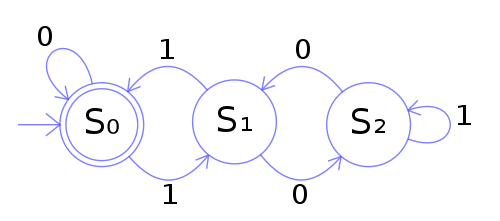
\includegraphics[height=4cm]{example.png}
		\end{center}
	\end{frame}

	\section{Formalizace výpočtu}
	\begin{frame}
		\frametitle{Formalizace výpočtu}
		\begin{block}{Konfigurace}
			Konfigurace KA je dvojice $(q , w) \in K \times \Sigma^*$, kde $q$ je aktuálny stav automatu a $w$ je doposud neprečtená část vstupného slova.
		\end{block}
		\begin{block}{Krok výpočtu}
			Krokem výpočtu KA je relace $\vdash_A$ na konfiguracích KA definovaná nasledovne: $(q, av) \vdash_A (p, v) \Longleftrightarrow p = \delta (q, a)$.
		\end{block}
		\begin{block}{Jazyk akceptovaný pomocí}
			Jazyk akceptovaný KA $A$ definujeme následovně:
			$L(A) = \{w \mid \exists\ p\in F:(q_0, w) \vdash_A^*(p,  \varepsilon)\}.$
		\end{block}
	\end{frame}

	\section{Typy konečných automatů}
	\begin{frame}
		\frametitle{Typy konečných automatů}
		\begin{exampleblock}{Mooreův stroj}
			Automat typu Moore je šestice $MO=\{S,I,\delta,0,lambda,\delta\}$. Změna na vstupu se u něj projeví na výstupu až v následujícím stavu. Výstupní funkce jsou tedy funkcemi pouze vnitřního stavu. Jeho obdobou je Mealyho automat.
		\end{exampleblock}
		\begin{exampleblock}{Mealyho stroj}
			Automat typu Mealy je šestice $\langle Z, Q, Y ,\Phi ,\Psi ,q\rangle$. Výstup je generován na základě příchozího vstupu i momentálního stavu, ve kterém se automat nachází. Stavový diagram automatu má ke každému přechodu přiřazenu nejen vstupní hodnotu, ale i výstupní hodnotu.
		\end{exampleblock}
	\end{frame}

	\section{Použité zdroje}
	\begin{frame}
		\frametitle{Použité zdroje}
		\begin{itemize}
			\item Konečný automat\\[0.3em]
			\scriptsize \url{https://cs.wikipedia.org/wiki/Konečný\_automat}\\
			\url{https://matematika.cz/konecny-automat}
			\url{https://sk.wikipedia.org/wiki/Konečný\_automat}\\
			\item \normalsize Mooreův stroj\\[0.3em]
			\scriptsize \url{https://cs.wikipedia.org/wiki/Mooreův\_stroj}\\
			\item \normalsize Mealyho stroj\\[0.3em]
			\scriptsize \url{https://cs.wikipedia.org/wiki/Mealyho_automat}\\
		\end{itemize}
	\end{frame}
\end{document}